\documentclass[12pt,a4paper]{article}
\usepackage[utf8x]{inputenc}
\usepackage{ucs}
\usepackage[spanish]{babel}
\usepackage{amsmath}
\usepackage{amsfonts}
\usepackage{amssymb}
\usepackage{makeidx}
\usepackage{graphicx}
\usepackage[width=17.00cm, height=23.00cm]{geometry}
\usepackage{hyperref}
\author{
	C411-Dalianys Pérez Perera\\C411-Dayany Alfaro González\\C411-Gilberto González Rodríguez
}
\date{}
\title{Mini proyecto de Clase Práctica 7 de Estadísticas}
\begin{document}
	\maketitle
	\section{Ejercicio 1}
	\textbf{a-)} Las variables independientes son el Mes y el Gasto, la variable dependiente las Ventas. El Mes está claro que es independiente. Con respecto al gasto y las ventas tiene más sentido que las ventas dependan del gasto puesto que, considerando que los gastos se realizan para aumentar la producción o para invertir en la calidad de los productos, las ventas de la empresa van a aumentar.
	
	\textbf{b-)} El modelo se realiza con la variable Gasto. El coeficiente de correlación entre Gasto y Ventas es 0.9988322 lo que implica que hay una relación líneal fuerte. Por lo tanto tiene sentido hacer la regresión lineal.\\
	Además el modelo de dispersión muesta la correlación lineal de ambas variables.\\
	\begin{center}
		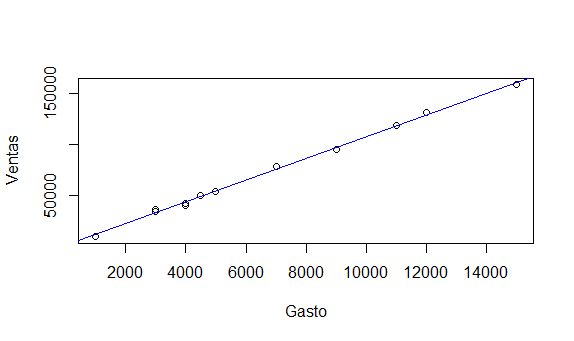
\includegraphics[scale=0.8]{images/GxV.png}
	\end{center}
	
	El summary de la regresión lineal simple en R es:\\
	
	Residuals:\\

	\begin{tabular}{cccccc}
		Min&     1Q& Median& Mean&     3Q&    Max\\
		-3385&  -2097&    258& 0& 1726&   3034 
	\end{tabular}\\ 
	
	Coefficients:\\

	\begin{tabular}{cccccc}
		 &     Estimate & Std. Error&     t value&   $Pr(>|t|)$&\\
		(Intercept) & 1383.4714 & 1255.2404 &  1.102  &  0.296&\\
		 Gasto      &   10.6222 &   0.1625  & 65.378  & 1.71e-14 &***\\
	\end{tabular}\\
	
	Signif. codes:  0 ‘***’ 0.001 ‘**’ 0.01 ‘*’ 0.05 ‘.’ 0.1 ‘ ’ 1\\
	
	Residual standard error: 2313 on 10 degrees of freedom\\
	
	Multiple R-squared:  0.9977,	Adjusted R-squared:  0.9974\\ 
	
	F-statistic:  4274 on 1 and 10 DF,  p-value: 1.707e-14\\
	
	Dada la gráfica de los residuos
	
	\begin{center}
		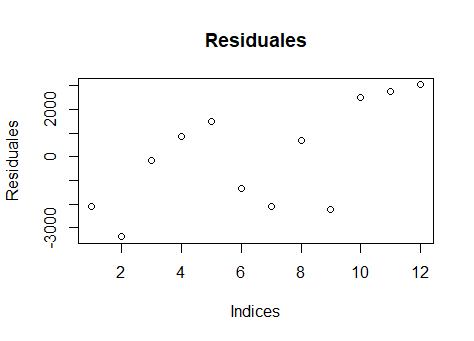
\includegraphics[scale=0.8]{images/PLOT1.png}
	\end{center}

	no queda muy claro a primera instancia qué pasa. Parece que no se cumplen los suspuestos dado que los datos están un poco dispersos, mas esta no está fácilmente identificable con ninguno de los 4 patrones vistos en Conferencia. Por lo tanto, para confirmar se procede a un análisis más detallado de la misma.
	
	De la columna Estimate en Coefficients se puede extraer que $\beta_0=1383.4714$ y $\beta_1=10.6222$, por lo que el modelo quedaría como:
	\begin{equation*}
	{Ventas}^{*} = 1383.4714 + Gasto * 10.6222
	\end{equation*}
	
	Sobre los coeficientes se puede decir que el intercepto es mucho mayor que el coeficiente de la variable independiente, esto quiere decir que hay gran parte de las Ventas de la población que no están explicadas a aprtir del Gasto, se pudieran hacer dos cosas, adicionar más variables al modelo, lo que se hará en el siguiente inciso, y en caso de no contar con más variables se puede realizar una transformación lineal y aplicar la regresón a las variables transformadas para obtener un valor más pequeño del intercepto. 
	El coeficiente del gasto es significativo al $0\%$, ya que su $Pr(>|t|)$ es $1.71e-14$, mucho menor que $0.05$, casi cero, mientras que el intercepto es significativo al $30\%$, lo cual es muy malo. Los coeficientes también indican que por cada unidad de incremento del Gasto se espera que las Ventas aumenten en $10.6$ unidades.\\
	
	Como el $Pr(>|t|)$ del gasto es menor que $0.05$ entonces el coeficiente sí está aportando al modelo, sin embargo el valor de $Pr(>|t|)$ para el intercepto es $0.296$, lo que implica que este no está aportando nada significativo al modelo.\\
	
	A pesar de que que R-cuadrado tiene más sentido analizarlo en un modelo de regresón múltiple, este valor cuanto más cercano a 1 mejor, en este caso es $0.997$, lo cual es bueno. El error estandar nos permite comparar este modelo con otros que tengan similares valores de R-cuadrado ajustado.\\ 
	
	Sin embargo dado que el p-valor de la prueba F, es menor que $0.05$ se puede concluir que al menos una variable es significativamente diferente de cero en el modelo.\\
	
	\textbf{Analizando los supuestos:}\\
	
	\textbf{Linealidad de los errores}\\
	Para analizar este supuesto se aplicó la prueba  Durbin-Watson obteniendo como resultado:
	 
	\begin{center}
		$DW = 1.1347$
		
		$p-valor = 0.03062$
		
		$\alpha = 0.05$
	\end{center}
	
	Por lo tanto como $p-valor < \alpha$ se puede rechazar la hipótesis nula y concluir que el supuesto no se cumple.\\
	
	\textbf{Valor esperado del error aleatorio igual a cero.}\\
	Como el valor esperado del error es 0, por lo tanto se cumple el supuesto, y con respecto al gráfico de los residuos se puede decir que los residuos están cercanos a cero en comparación con los valores ajustados que son mucho más grandes.
	
	\begin{center} 
		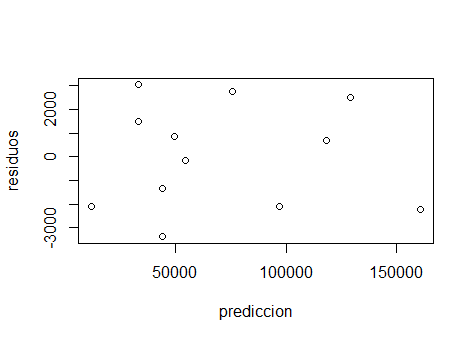
\includegraphics[scale=0.8]{./images/PLOT2.png}
	\end{center}
	
	\textbf{Homocedasticidad}\\
	Para analizar este supuesto se aplicó la prueba Breusch-Pagan obteniendo como resultado:
	
	\begin{center}
		$BP = 0.018699$
		
		$p-valor = 0.8912$
		
		$\alpha = 0.05$
	\end{center}
	
	
	Interpretación: Como $p-valor > \alpha$ no se puede rechazar $H_0$ por lo que se puede decir que se cumple la homocedasticidad.\\
	
	\textbf{Los errores además de ser independientes son idénticamente distribuidos y siguen distribución normal con media cero y varianza constante.}\\
	Analizando el test de contraste de normalidad Shapiro-Wilk:
	\begin{center}
		$W = 0.92894$ \\
		$p-valor = 0.369$\\
		$\alpha = 0.05$
	\end{center}
	Interpretación: Como $p-valor > \alpha$ no se puede rechazar la hipótesis nula por tanto los errores siguen una distribución normal.
	
	Para constatar este resultado también se puede observar el histograma de frecuencias y los cuantiles normales.
	
	\begin{center}
		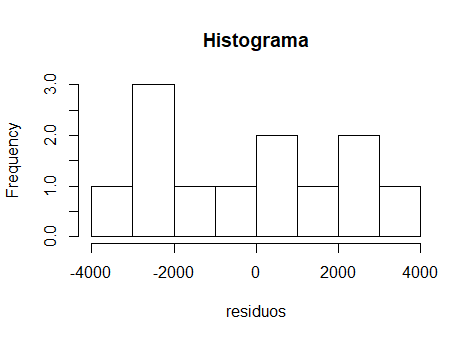
\includegraphics[width=4in]{./images/PLOT3.png}
	\end{center}
	
	\begin{center}
		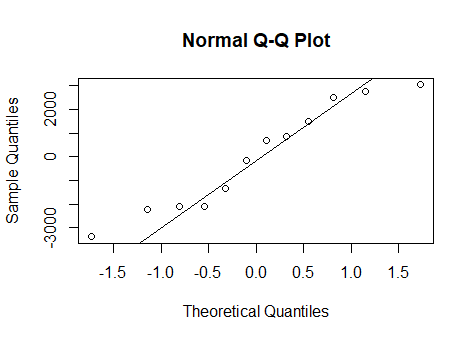
\includegraphics[width=4in]{./images/PLOT4.png}
	\end{center}
	
	Por lo tanto se puede concluir que este modelo de regresión lineal simple no es muy bueno para hacer predicciones ya que no cumple con el supuesto de linealidad.\\

	\textbf{c-)} Regresión lineal múltiple
	El coeficiente de correlación entre Gasto y Ventas es 0.9988322 como se habia visto en b-), indicando una relación lineal fuerte, y entre Ventas y Mes el coeficiente es 0.5573783, indicando aunque débil, cierta relación. Por lo tanto tiene sentido plantear el modelo.
	
	El summary de la regresión lineal múltiple en R es:\\
	
	Residuals:\\
	
	\begin{tabular}{cccccc}
		Min&     1Q& Median& Mean&     3Q&    Max\\
		-1793.73&  -1558.33& -1.73&    0.00&   1374.19&   1911.58  
	\end{tabular}\\ 
	
	Coefficients:\\
	
	\begin{tabular}{cccccc}
		&     Estimate & Std. Error&     t value&   $Pr(>|t|)$&\\
		(Intercept) & -567.6098 & 1041.8836 &  -0.545  &  0.59913&\\
		Gasto      &   10.3825 &   0.1328  & 78.159  & 4.65e-14 &***\\
		Mes      &   541.3736 &   158.1660  & 3.423  & 0.00759 &**\\
	\end{tabular}\\
	
	Signif. codes:  0 ‘***’ 0.001 ‘**’ 0.01 ‘*’ 0.05 ‘.’ 0.1 ‘ ’ 1\\
	
	Residual standard error: 1607 on 9 degrees of freedom\\
	
	Multiple R-squared:  0.999,	Adjusted R-squared:  0.9988\\
	 
	F-statistic:  4433 on 2 and 9 DF,  p-value: 3.368e-14\\
	
	El $Pr(>|t|)$ del intercepto es elevado con 0.59913, o sea que es significativo al $60\%$, muy malo. El valor del R-squared es muy bueno, casi 1. El p-valor de la prueba F, es menor que $0.05$ por lo que se puede decir que al menos una variable es significativamente diferente de cero en el modelo.\\
	
	\textbf{Analizando los supuestos:}\\
	
	\textbf{Linealidad de los errores}\\
	Para analizar este supuesto se aplicó la prueba  Durbin-Watson obteniendo como resultado:
	
	\begin{center}
		$DW = 2.1077$
		
		$p-valor = 0.3133$
		
		$\alpha = 0.05$
	\end{center}
	
	Por lo tanto como $p-valor > \alpha$ no se puede rechazar la hipótesis nula y se concluye que el supuesto se cumple.\\
	
	\textbf{Valor esperado del error aleatorio igual a cero.}\\
	Como el valor esperado esperado del error es 0.00 entonces se cumple el supuesto
	
	\textbf{Homocedasticidad}\\
	Para analizar este supuesto se aplicó la prueba Breusch-Pagan obteniendo como resultado:
	
	\begin{center}
		$BP = 2.7174$
		
		$p-valor = 0.257$
		
		$\alpha = 0.05$
	\end{center}
	
	Interpretación: Como $p-valor > \alpha$ no se puede rechazar $H_0$ por lo que se puede decir que se cumple la homocedasticidad.\\
	
	Además para comprobar lo anterior se puede consultar los gráficos de los residuos 
	
	\begin{center}
		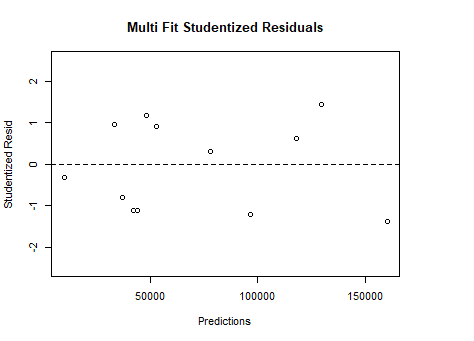
\includegraphics[width=4in]{./images/MFDR1.png}
	\end{center}
	
	\begin{center}
		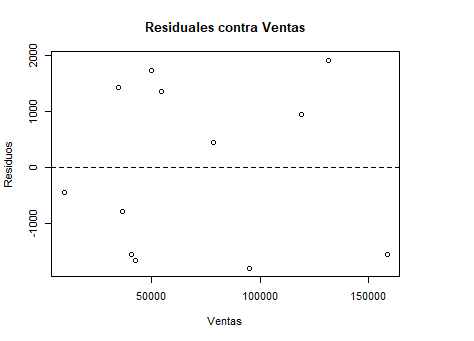
\includegraphics[width=4in]{./images/RVV1.png}
	\end{center}
	
	\textbf{Los errores además de ser independientes son idénticamente distribuidos y siguen distribución normal con media cero y varianza constante.}\\
	Analizando el test de contraste de normalidad Shapiro-Wilk:
	\begin{center}
		$W = 0.92894$ \\
		$p-valor = 0.369$\\
		$\alpha = 0.05$
	\end{center}
	Interpretación: Como $p-valor > \alpha$ no se puede rechazar la hipótesis nula por tanto los errores siguen una distribución normal.
	
	Para constatar este resultado también se puede observar el histograma de frecuencias y los cuantiles normales.
	
	\begin{center}
		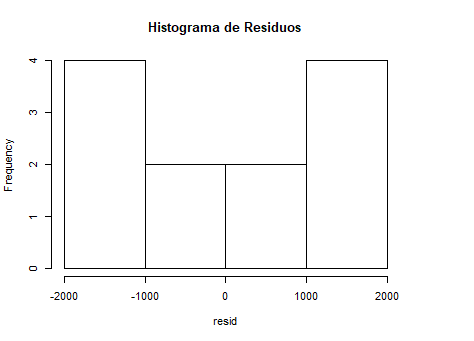
\includegraphics[width=4in]{./images/HR1.png}
	\end{center}
	
	\begin{center}
		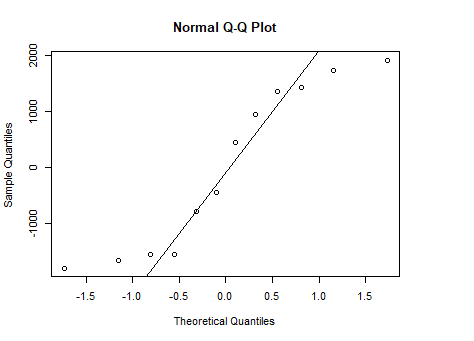
\includegraphics[width=4in]{./images/QQPLOT1.png}
	\end{center}
	
	\textbf{Las variables independientes del modelo no están correlacionadas.}\\
	El coeficiente de correlación entre Gasto y Mes es $0.5271186$, por lo que si consideramos que hay correlación esta es muy débil, por lo tanto no es tan malo para el modelo, aunque no es ideal.
	
	Por lo tanto se pudiera decir que este modelo de regresión lineal múltiple es bastante bueno para hacer predicciones si se tiene en cuenta el buen valor de R-cuadrado ajustado y se acepta que el nivel de correlación entre las variables dependientes, aunque no es ideal dado esto último.
	
	 \textbf{d-)} Comparando ambos modelos. Se puede concluir que los coeficientes mejoran en el modelo múltiple, aunque estos están lejos de ser ideales, implicando que la incluso de la variable Mes ayuda en la explicación de la variable dependiente a partir de las independientes. Los valores de R-cuadrado son muy similares. La principal diferencia es que el modelo múltiple cumple con el supuesto de la linealidad de los errores, mientras que el simple no lo hace. Aunque el modelo múltiple parece más apropiado para hacer predicciones que el simple, de manera general, habría que valorar el supuesto adicional para el caso de los modelos múltiples, relacionado con la independencia de las variables independientes, puesto que el coeficiente de correlación no es el ideal para asumir la no correlación entre estas.   
	
	\section{Ejercicio 3}
	Realizando la regresión lineal múltiple con todas las variables independientes,
	la formúla:
	\begin{center}
		sales $\sim$ newspaper + TV + radio 
	\end{center}
	
	{\bf summary: }\\
	
	Residuals:\\
	
	\begin{tabular}{ccccc}
		Min&     1Q& Median& 3Q&    Max\\
		-8.8277& -0.8908&  0.2418&  1.1893&  2.8292 
	\end{tabular}\\ 
	
	Coefficients:\\
	
	\begin{tabular}{cccccc}
		&     Estimate & Std. Error&     t value&   $Pr(>|t|)$&\\
		(Intercept) & 2.938889 &  0.311908 &  9.422  & $<2e-16$ &***\\
		newspaper   &-0.001037 &  0.005871 & -0.177  &   0.86 &\\ 
		radio       & 0.188530 &  0.008611 & 21.893  & $<2e-16$ &***\\
		TV          & 0.045765 &  0.001395 & 32.809  &$<2e-16$ &***\\
	\end{tabular}\\
	
	Signif. codes:  0 ‘***’ 0.001 ‘**’ 0.01 ‘*’ 0.05 ‘.’ 0.1 ‘ ’ 1\\
	
	Residual standard error: 1.686 on 196 degrees of freedom\\
	
	Multiple R-squared:  0.8972,	Adjusted R-squared:  0.8956\\
	 
	F-statistic: 570.3 on 3 and 196 DF,  p-value: < 2.2e-16\\
	
	Análisis de supuestos:\\
	
	\textbf{Linealidad de los errores}
	\begin{center}
		$DW = 2.1077$
		
		$p-valor = 0.3133$
		
		$\alpha = 0.05$
	\end{center}
	El $p-valor > \alpha$ por lo tanto se cumple el supuesto.\\
	
	\textbf{Valor esperado del error aleatorio igual a cero.}\\
	Media de los errores = $-4.893438e-17$\\
	Suma de los errores = $-9.756085e-15$\\
	Por lo tanto se cumple el supuesto.\\
	
	\textbf{Homocedasticidad}\\
	\begin{center}
		$BP = 5.1329$
		
		$p-valor = 0.1623$
		
		$\alpha = 0.05$
	\end{center}
	El $p-valor > \alpha$ por lo tanto se cumple el supuesto.\\
	
	\textbf{Los errores además de ser independientes son idénticamente distribuidos y siguen distribución normal con media cero y varianza constante.}\\
	Analizando el test de contraste de normalidad Shapiro-Wilk:
	\begin{center}
		$W = 0.87303$ \\
		$p-valor = 0.07141$\\
		$\alpha = 0.05$
	\end{center}
	El $p-valor > \alpha$ por lo tanto se cumple el supuesto.\\
	
	\textbf{Las variables independientes del modelo no están correlacionadas.}\\
	Los coeficientes de correlación son:\\
	Entre TV y radio $0.05480866$.\\
	Entre TV y newspaper $0.05664787$\\
	Entre radio y newspaper $0.3541038$\\
	Todos están entre $-0.4$ y $0.4$ por lo tanto no hay correlación y se cumple el supuesto.\\
	
	El $Pr(>|t|)$ para newspaper es muy malo, con 0.86, indicando poca significación de esta variable para el modelo, por lo que para seguir el enfoque backward este es la variable que se decide eliminar para volver a realizar el modelo. El R-cuadrado no es ideal pero es bastante bueno, y todos los supuestos se cumplen, por lo tanto el modelo en sí ya está bastante bien ajustado a los datos.\\
	
	Analizando el modelo sin la variable newspaper, la fórmula:
	\begin{center}
		sales $\sim$ TV + radio 
	\end{center}
	
	{\bf summary: }\\
	
	Residuals:\\
	
	\begin{tabular}{ccccc}
		Min&     1Q& Median& 3Q&    Max\\
		-8.7977& -0.8752&  0.2422&  1.1708&  2.8328 
	\end{tabular}\\ 
	
	Coefficients:\\
	
	\begin{tabular}{cccccc}
		&     Estimate & Std. Error&     t value&   $Pr(>|t|)$&\\
		(Intercept) & 2.938889 &  0.311908 &  9.422  & $<2e-16$ &***\\
		(Intercept) & 2.92110  &  0.29449  & 9.919   & $<2e-16$ &***\\
		radio       & 0.18799  &  0.00804  & 23.382  & $<2e-16$ &***\\
		TV          & 0.04575  &  0.00139  & 32.909  & $<2e-16$ &***\\
	\end{tabular}\\
	
	Residual standard error: 1.681 on 197 degrees of freedom
	Multiple R-squared:  0.8972,	Adjusted R-squared:  0.8962 
	F-statistic: 859.6 on 2 and 197 DF,  p-value: < 2.2e-16
	
	Análisis de supuestos:\\
	
	\textbf{Linealidad de los errores}
	\begin{center}
		$DW = 2.1077$
		
		$p-valor = 0.3133$
		
		$\alpha = 0.05$
	\end{center}
	El $p-valor > \alpha$ por lo tanto se cumple el supuesto.\\
	
	\textbf{Valor esperado del error aleatorio igual a cero.}\\
	Media de los errores = $5.603157e-18$\\
	Suma de los errores = $1.110223e-15$\\
	Por lo tanto se cumple el supuesto.\\
	
	\textbf{Homocedasticidad}\\
	\begin{center}
		$BP = 4.8093$
		
		$p-valor = 0.0903$
		
		$\alpha = 0.05$
	\end{center}
	El $p-valor > \alpha$ por lo tanto se cumple el supuesto.\\
	
	\textbf{Los errores además de ser independientes son idénticamente distribuidos y siguen distribución normal con media cero y varianza constante.}\\
	Analizando el test de contraste de normalidad Shapiro-Wilk:
	\begin{center}
		$W = 0.87303$ \\
		$p-valor = 0.07141$\\
		$\alpha = 0.05$
	\end{center}
	El $p-valor > \alpha$ por lo tanto se cumple el supuesto.\\
	
	\textbf{Las variables independientes del modelo no están correlacionadas.}\\
	El coeficiente de correlación entre TV y radio es $0.05480866$.\\
	Como está entre $-0.4$ y $0.4$ entonces no hay correlación y se cumple el supuesto.\\
	
	El R-cuadrado ajustado aumentó ligeramente y se siguen cumpliendo todos los supuestos, por lo que efectivamente se comprueba que la variable newspaper no era significativa para el modelo. En este punto no se observa ninguna otra característica relevante para eliminar otra de las variables independientes, no obstante a modo de investigación este analisis se hizo elimando TV y radio, obteniendose en ambos casos valores muy ceranos a cero del R-cuadrado y fallo del supuesto de homocedasticidad. Por lo tanto se puede concluir que este último modelo es el que más se ajusta a los datos.\\
	
	
%	\textbf{Linealidad de los errores}\\
%	\textbf{Valor esperado del error aleatorio igual a cero.}\\
%	\textbf{Homocedasticidad}\\
%	\textbf{Los errores además de ser independientes son idénticamente distribuidos y siguen distribución normal con media cero y varianza constante.}\\
%	\textbf{Las variables independientes del modelo no están correlacionadas.}\\
	
		
\end{document}